\documentclass[a4paper,12pt]{report}
\usepackage{graphicx}
\graphicspath{{picaa/}}
\usepackage{listings}
\usepackage{amsmath}
\usepackage[T2A]{fontenc}
\usepackage[utf8]{inputenc}
\usepackage[english,russian]{babel}
\usepackage{pgfplots} 

\usepackage{longtable}
\usepackage{geometry}
\geometry{left=2cm}
\geometry{right=1.5cm}
\geometry{top=1cm}
\geometry{bottom=2cm}
\lstset{language = C++,
	keywordstyle = \color{orange},
	stringstyle = \color{green},
	commentstyle = \color{red},
	columns = fullflexible
}

\begin{document}

    \begin{titlepage}

        \begin{center}
            \large
            \textbf{Государственное образовательное учреждение высшего профессионального образования\\
            “Московский государственный технический университет имени Н.Э.Баумана”\\}
            
\includegraphics{bmstu-logo.png}
			\vspace{1cm}
            
            \textsc{Дисциплина: Анализ алгоритмов}
            \vspace{0.5cm}
                
            \textsc{Лабораторная работа №6}
            \vspace{1cm}
            
            {\LARGE \textbf{Исследование эвристических алгоритмов на основе муравьиного алгоритма}}
            \vspace{3cm}
                    
            \begin{flushright}
            	Студент группы ИУ7-55Б,\\   
            	Руднев К. К.,\\
            	\vspace{0.5cm}
            	Преподаватель,\\
            	Волкова Л. Л.,\\
            	Строганов Ю. В.
            	
            \end{flushright}
            \vfill
            
            2019 г.
            
            \end{center}

    \end{titlepage}

	\setcounter{page}{2}
	\tableofcontents
    \chapter*{Введение}

    	Задача коммивояжёра — одна из самых известных задач комбинаторной оптимизации, заключающаяся в поиске самого выгодного маршрута, проходящего через указанные города хотя бы по одному разу с последующим возвратом в исходный город \cite{commi2}.
    	Задача коммивояжёра относится к числу транс вычислительных: уже при относительно небольшом числе городов (66 и более) она не может быть решена методом перебора вариантов никакими теоретически мыслимыми компьютерами за время, меньшее нескольких миллиардов лет.
    	Муравьиный алгоритм — один из эффективных полиномиальных алгоритмов для нахождения приближённых решений задачи коммивояжёра, а также решения аналогичных задач поиска маршрутов на графах. 
    	Суть подхода заключается в анализе и использовании модели поведения муравьёв, ищущих пути от колонии к источнику питания, и представляет собой метаэвристическую оптимизацию.\\

		Цель работы: изучить муравьиный алгоритм на материале решения задачи коммивояжёра.\\
		
		Задачи:
		\begin{itemize}
			\item описать реализацию, реализовать метод;
			\item выбрать класс данных, составить набор данных;
			\item провести параметризацию метода на основании муравьиного алгоритма   для выбранного класса данных.
		\end{itemize}

    \label{sec:intro}

    \newpage

    \chapter{Аналитическая часть}
        \label{sec:analitic_part}

        	В рамках раздела будет дано аналитическое описание алгоритма для решения задачи коммивояжёра - алгоритма полного перебора и муравьиного алгоритма.
        	
	\section{Алгоритм рекурсивного полного перебора}

   			Полный перебор — метод решения математических задач. 
   			Относится к классу методов поиска решения исчерпыванием всевозможных вариантов. 
   			Сложность полного перебора зависит от количества всех возможных решений задачи. 
   			Если пространство решений очень велико, то полный перебор может не дать результатов в течение нескольких лет или даже столетий \cite{commi}. 
   			Полный перебор гарантировано дает идеальное решение, так как гарантируется, что каждый вариант будет рассмотрен.
   			
   			Однако на практике этот  алгоритм не применяется, так как чаще необходимо получить, возможно, не самое лучшее решение, но за минимальное время.

	\section{Муравьиный алгоритм}

   			Муравьиный алгоритм — один из эффективных полиномиальных алгоритмов для нахождения приближённых решений задачи коммивояжёра. 
   			В основе алгоритма лежит поведение муравьиной колонии — маркировка более удачных путей большим количеством феромона\cite{ant1}.
   			\newline
   			Введем математическую модель.
   			У муравья есть 3 чувства:
   			
   			\begin{enumerate}
   				\item зрение (муравей может оценить длину ребра);
   				\item обоняние (муравей может учуять феромоны);
   				\item память(муравей запоминает свой маршрут).
   			\end{enumerate}
   		
   			Благодаря феромонам и обонянию муравьи могут обмениваться информацией, имеет место непрямой обмен информацией \cite{shtovba}.
   			Введем вероятность $P_{k, ij}(t)$.
   			Она будет определяться по следующему правилу выбора существующего города j муравьем k, находящимся в городе i:
   			
   			\begin{equation}
   				P_{k, ij}(t)=
   				{\frac {(\tau _{i,j}^{\alpha })(\eta _{i,j}^{\beta })}{\sum (\tau _{i,j}^{\alpha })(\eta _{i,j}^{\beta })}}
   			\end{equation}
   			где \quad$ \tau _{i,j} - $ расстояние от города i до j;
   			
   			$\eta _{i,j} - $количество феромонов на ребре ij;
   			$\alpha - $ параметр влияния длины пути;
   			$\beta - $ параметр влияния феромона.
   			В случае, если муравей уже посетил j-ый город, то $P_{k, ij}(t) = 0$
   			
   			\vspace{0.5cm}
   			После того, как муравей успешно проходит маршрут, он оставляет на всех пройденных ребрах след, обратно пропорциональный длине пройденного пути. Итого, новый след феромона вычисляется по формуле \ref{form:eva}:
   			\begin{equation}\label{form:eva} 
   			\tau _{i,j}=(1-\rho )\tau _{i,j}+\Delta \tau _{i,j},
   			\end{equation}
   			где \quad$ \rho _{i,j}$ - \text{доля феромона, который испарится;} 
   			
   			$\tau _{i,j}$ - \text{количество феромона на дуге ij;} 
   			
   			$\Delta \tau _{i,j}$ - \text{количество отложенного феромона, вычисляется по формуле \ref{form:add1}.}
   	
   		\newpage
   	
   		\section{Муравьиный алгоритм в задаче коммивояжёра}

   			Рассмотрим, как реализовать четыре составляющие самоорганизации муравьев при оптимизации маршрута коммивояжера. 
   			Многократность взаимодействия реализуется итерационным поиском маршрута коммивояжера одновременно несколькими муравьями. 
   			При этом каждый муравей рассматривается как отдельный, независимый коммивояжер, решающий свою задачу. 
   			За одну итерацию алгоритма каждый муравей совершаетполный маршрут коммивояжера. 
   			Положительная обратная связь реализуется как имитация поведения муравьев типа «оставление следов – перемещение по следам». 
   			Чем больше следов оставлено на тропе — ребре графа в задаче коммивояжера, тем больше муравьев будет передвигаться по ней. 
   			При этом на тропе появляются новые следы, привлекающие дополнительных муравьев. 
   			Для задачи коммивояжера положительная обратная связь реализуется следующим стохастическим правилом: вероятность включения ребра графа в маршрут муравья пропорциональна количеству феромона на нем.
   			
   			\vspace{0.5cm}
   			Теперь с учетом особенностей задачи коммивояжёра, мы можем описать локальные правила поведения муравьев при выборе пути:\
   			
   			\begin{enumerate}
   			\item Муравьи имеют собственную «память». Поскольку каждый город может быть посещён только один раз, то у каждого муравья есть список уже посещенных городов - список запретов. Обозначим через $J$ список городов, которые необходимо посетить муравью $k$ , находящемуся в городе $i$;
   			
   			\item Муравьи обладают «зрением» - видимость есть эвристическое желание посетить город $j$ , если муравей находится в городе $i$ . Будем считать, что видимость обратно пропорциональна расстоянию между городами; 
   			
   			\item Муравьи обладают «обонянием» - они могут улавливать след феромона, подтверждающий желание посетить город $j$ из города $i$ на основании опыта других муравьёв. Количество феромона на ребре $(i,j)$ в момент времени $t$ обозначим через  $\tau _{i,j} (t)$ ;
   			
   			\item На этом основании мы можем сформулировать вероятностнопропорциональное правило, определяющее вероятность перехода $k$-ого муравья из города $i$  в город $j$;
   			
   			\item Пройдя ребро $(i,j)$ , муравей откладывает на нём некоторое количество феромона, которое должно быть связано с оптимальностью сделанного выбора.
   			\end{enumerate}
   			
   			Пусть $T _{k} (t)$ есть маршрут, пройденный муравьем $k$ к моменту времени $t$ , $L _{k} (t)$ - длина этого маршрута, а $Q$ - параметр, имеющий значение порядка длины оптимального пути. Тогда откладываемое количество феромона может быть задано в виде:
   			
   			\begin{equation}\label{form:add} 
   			{\displaystyle \Delta \tau _{i,j}^k={\begin{cases}Q/L_{k}& {\mbox{Если k-ый мурваей прошел по ребру ij;}}\\0&{\mbox{Иначе}}\end{cases}}}
   			\end{equation}
   			где \quad Q - количество феромона, переносимого муравьем;
   			
   			Тогда
   			\begin{equation}\label{form:add1} 
   			\Delta \tau _{i,j}= \tau _{i,j}^0 + \tau _{i,j}^1 + ... + \tau _{i,j}^k 
   			\end{equation}
   			
   			где k - количество муравьев в вершине графа с индексами i и j.

	\section{Вывод}

    		В данном разделе были рассмотрены общие принципы муравьиного алгоритма и применение его к задаче коммивояжера. 

    \newpage

    \chapter{Конструкторская часть}
        \label{sec:construct_part}
 
        	В рамках раздела будут представлены схемы полного перебора и муравьиного алгоритмов, изображенные на рисунках \ref{ris:full}-\ref{ris:muravei}

	\section{Разработка алгоритмов}
	
		\begin{figure}[h!]
			\centering
			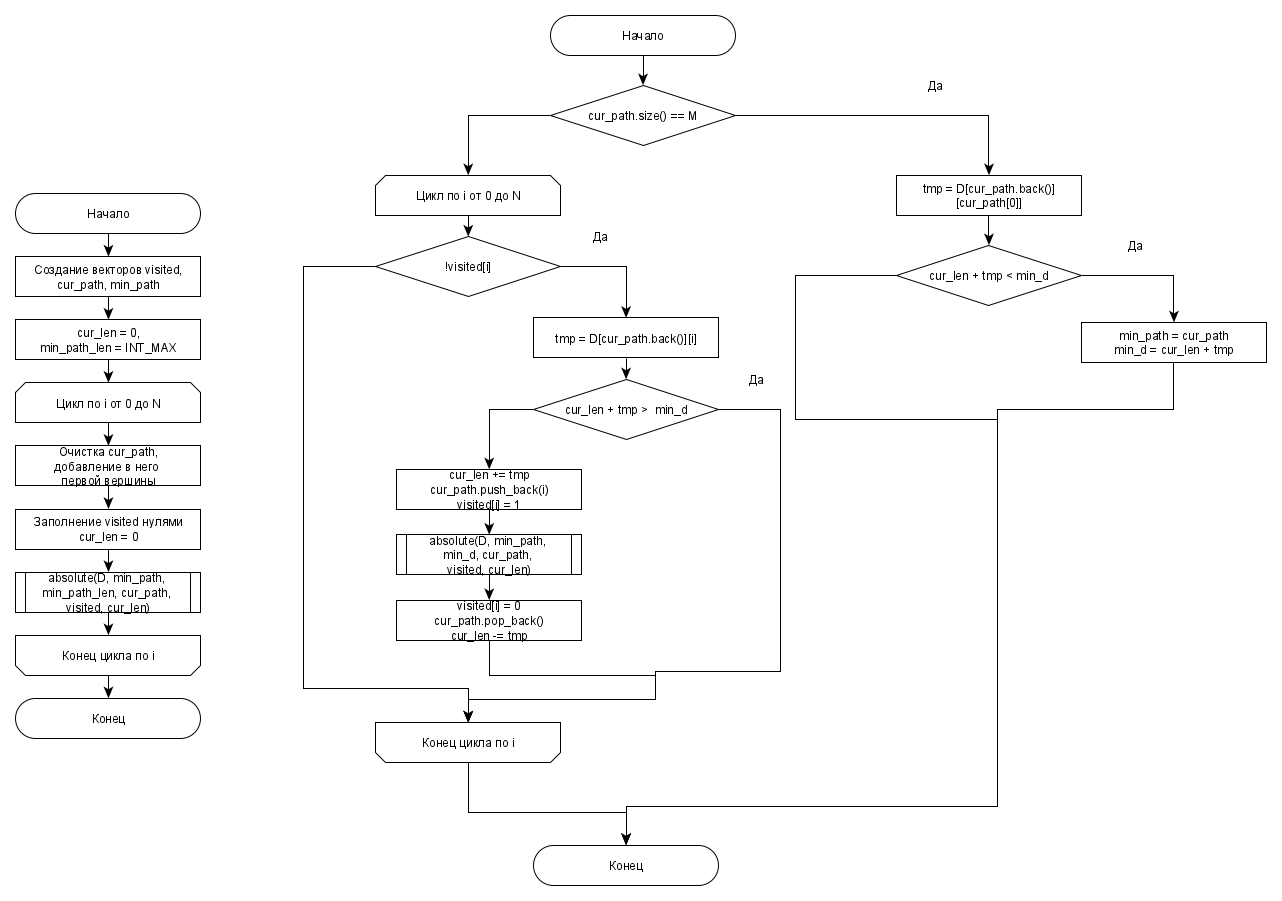
\includegraphics[width=1.05\linewidth]{full1.png}
			\caption{Алгоритм полного перебора}
			\label{ris:full}
		\end{figure}
		
		\newpage
		
		\begin{figure}[h!]
			\centering
			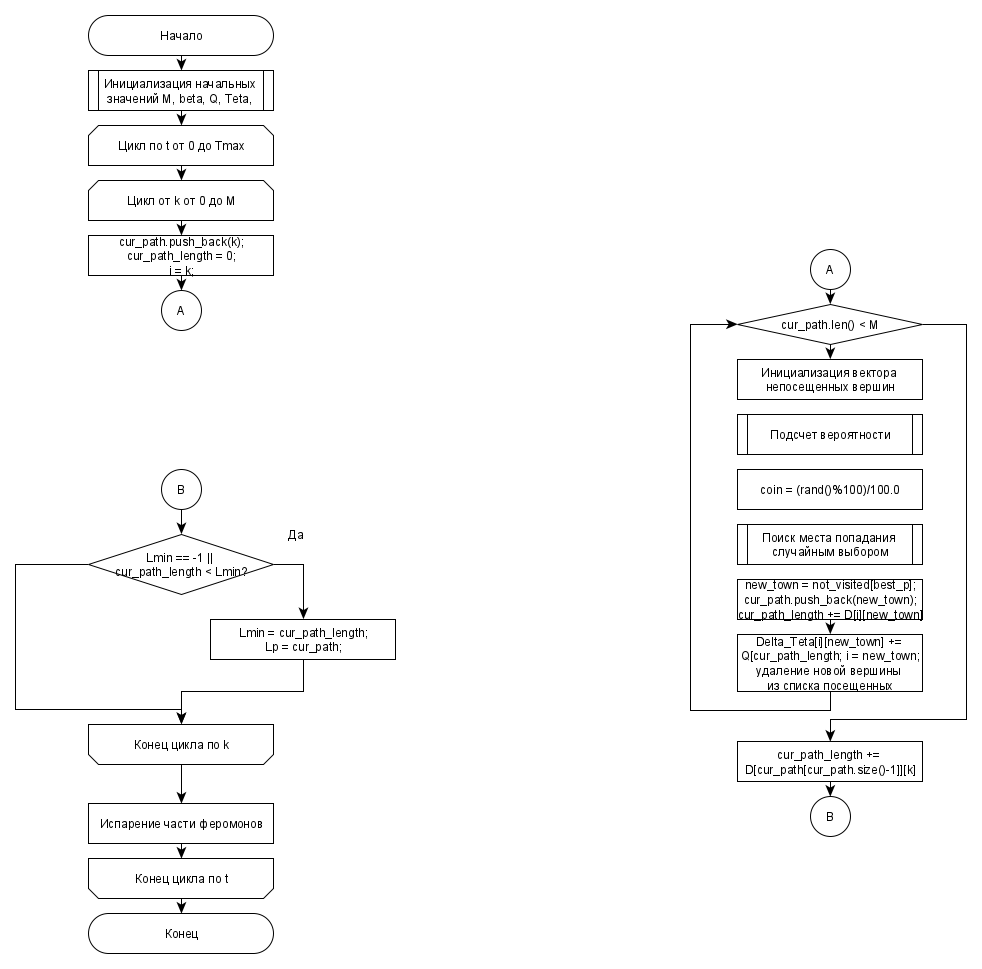
\includegraphics[width=1\linewidth]{muravei2.png}
			\caption{Муравьиный алгоритм}
			\label{ris:muravei}
		\end{figure}
	
	\section{Вывод}

			В данном разделе были рассмотрены схемы полного перебора и муравьиного алгоритмов.

    \newpage

    \chapter{Технологическая часть}
        \label{sec:tecnologic_part}

        	Замеры времени были произведены на: Intel(R) Core(TM) i7-8565U, 4 ядра, 8 логических процессоров.

	\section{Средства реализации}

			Для реализации алгоритмов использовался язык программирования C++ 11 и среда разработки QtCreator Community Edition 5.5.
			 
			Замер времени реализован с помощью метода high\_resolution\_clock() класса std::chrono.
			
			Измеряется время исполнения кода чистого алгоритма (без учета времени на создание матриц, генерацию данных и т.п.).\\

	\section{Требования к программному обеспечению}

			На вход программа должна получать граф, представленный матрицей смежностей. 
			
			Граф должен иметь хотя бы 2 вершины. 
			При полном переборе программа должна возвращать кратчайший путь в графе.

	\section{Листинг кода}

        	На листинге \ref{list:etc} представлены дополнительные функции и объявления, необходимые для реализации алгоритмов.
        	На листинге \ref{list:seq_wino} представлена реализация алгоритма полного перебора.
        	На листинге \ref{list:par_wino} представлена реализация муравьиного алгоритма.\\
        	
        	\begin{lstlisting}[frame = single, breaklines, caption =  Вспомогательные классы и объявления, label=list:etc]
        #include <algorithm>
        #include <chrono>
        #include <ctime>
        #include <cstdlib>
        #include <iostream>
        #include <limits>
        #include <math.h>
        #include <stdlib.h>
        #include <vector>
        
        #define MAX_CITY 10
        #define MAX_L 15
        #define MIN_L 1
        
        #define ALPHA 0.75
        #define BETHA (1 - ALPHA)
        #define RO 0.25
        #define QU (MAX_CITY * MAX_L)
        
        template <class t>
        t** create_mat(int m, int n)
        {
        	t** mat = new t* [m];
        
        	for (int i = 0; i < m; ++i)
        		mat[i] = new t[n];
        
        	return mat;
        }
        
        struct Ant
        {
        public:
        	Ant(int i):
        	start_city(i), cur_city(i), Lk(0)
        	{
        		route = new int[MAX_CITY];
        		Jk = new float[MAX_CITY];
        	}
        
        	void show_route()
        	{
        		for (int i = 0; i < MAX_CITY; ++i)
        			printf("%d\t", route[i]);
        	}
        
        	bool city_passed(int c)
        	{
        		for (int i = 0; i < MAX_CITY; ++i)
        			if (c == route[i])
        				return true;
        		return false;
        	}
        
        	int start_city;
        	int cur_city;
        	int Lk;
        
        	int* route;
        	float* Jk;
        };
        	\end{lstlisting}
        	
        	\begin{lstlisting}[frame = single, breaklines, caption = Алгоритм полного перебора, label=list:seq_wino]
	void perebor(bool output = true)
	{
		std::pair <int, std::vector<int>> res = this->absolute_find();
		min_path_full = res.second;
		min_length_full = res.first;
	
		if (output)
		{
			std::cout << "\nFull perebor:\n";
			get_result<std::vector<int>>(min_path_full, min_length_full);
		}
	}
	
	std::pair <int, std::vector<int>> absolute_find()
	{
		int n = MAX_CITY;
		std::vector<bool> visited(n, 0);
		std::vector<int> cur_path;
		std::vector<int> min_path;
		int cur_len = 0;
		int min_path_len = INT_MAX;
		for (int i = 0; i < n; i++)
		{
			cur_path.clear();
			cur_path.push_back(i);
			fill(visited.begin(), visited.end(), 0);
			visited[i] = 1;
			cur_len = 0;
			absolute(min_path, min_path_len, cur_path, visited, cur_len);
		}
		return std::pair<int, std::vector<int>>(min_path_len, min_path);
	}
	
	void absolute(std::vector<int> &min_path, int &min_d, std::vector<int> &cur_path, std::vector<bool> &visited, int &cur_len)
	{
		size_t M = MAX_CITY;
		if (cur_path.size() == M)
		{
			ss++;
			int tmp = cities[cur_path.back()][cur_path[0]];
			if (cur_len + tmp < min_d)
			{
				min_path = cur_path;
				min_d = cur_len + tmp;
			}
			return;
		}
		for (size_t i = 0; i < M; i++)
		{
			if (!visited[i])
			{
				int tmp = cities[cur_path.back()][i];
				if (cur_len + tmp > min_d)
					continue;
				cur_len += tmp;
				cur_path.push_back(i);
				visited[i] = 1;
				absolute(min_path, min_d, cur_path, visited, cur_len);
				visited[i] = 0;
				cur_path.pop_back();
				cur_len -= tmp;
			}
		}
	}
        	\end{lstlisting}
        	
        	\begin{lstlisting}[frame = single, breaklines, caption = Муравьиный алгоритма, label=list:par_wino]
	    void muravei(float a, float r, int tm, bool output = true)
	    {
	    	alfa=a;
	    	betha=1 - a;
	    	ro=r;
	    	tmax=tm;
	    	create_colony();
	    
	    	float** vision = create_mat<float>(MAX_CITY, MAX_CITY);
	    	for (int i = 0; i < MAX_CITY; ++i)
	    	{
	    		for (int j = i; j < MAX_CITY; ++j)
	    		{
	    			if (i != j)
	    			{
	    				vision[i][j] = (float)1/cities[i][j];
	    				vision[j][i] = vision[i][j];
	    			}
	    			else
	    			{
	    				vision[i][j] = 0;
	    			}
	    		}
	    	}
	    
	    	float** substance = create_mat<float>(MAX_CITY, MAX_CITY);
	    	for (int i = 0; i < MAX_CITY; ++i)
	    	{
	    		for (int j = 0; j < MAX_CITY; ++j)
	    		{
	    			substance[i][j] = 0.5;
	    		}
	    	}
	    
	    	float** weight = create_mat<float>(MAX_CITY, MAX_CITY);
	    	recalc_weight(weight, substance, vision);
	    
	    	float** delta_substance = create_mat<float>(MAX_CITY, MAX_CITY);
	    	for (int i = 0; i < MAX_CITY; ++i)
	    	{
	    		for (int j = 0; j < MAX_CITY; ++j)
	    		{
	    			delta_substance[i][j] = 0;
	    		}
	    	}
	    
	    	min_length = std::numeric_limits<int>::max();
	    
	    	for (int t = 0; t < tmax; ++t)
	    	{
	    		for (unsigned int i = 0; i < MAX_CITY; ++i)
	    		{
	    			set_ant(ants_colony[i]);
	    			move_ant(ants_colony[i], weight, substance, QU);
	    		}
	    
	    		int best = -1;
	    		for (unsigned int i = 0; i < MAX_CITY; i++)
	    			if (ants_colony[i]->Lk < min_length)
	    			{
	    				best = i;
	    				min_length = ants_colony[i]->Lk;
	    			}
	    
	    		if (best != -1)
	    			copy_array<int*, int*>(min_path, ants_colony[best]->route);
	    
	    		recalc_substance(substance, delta_substance);
	    		recalc_weight(weight, substance, vision);
	    	}
	    
	    	min_length += cities[min_path[MAX_CITY-1]][min_path[0]];
	    
	    	if (output)
	    	{
	    		std::cout << "\nMuravey:\n";
	    		get_result<int*>(min_path, min_length);
	    	}
	    }
	    
	    void create_colony()
	    {
	    	for (int i = 0; i < MAX_CITY; i++)
	   	{
	    		Ant* ant = new Ant(i);
	    		ants_colony.push_back(ant);
	    	}
	    }
	    
	    void set_ant(Ant* &ant)
	    {
	    	int start = ant->start_city;
	    	ant->cur_city = start;
	    	ant->Lk = 0;
	    	for (int i = 0; i < MAX_CITY; i++)
	    	{
	    		ant->route[i] = -1;
	    		ant->Jk[i] = 1;
	    	}
	    
	    	ant->route[0] = start;
	    	ant->Jk[start] = 0;
	    }
	    
	    int choose_next(float* prob)
	    {
	    	int i = 0;
	    	srand(time(nullptr));
	    	float r = (float)(rand())/RAND_MAX;
	    
	    	if (r == 0.)
	    	{
	    		while (prob[i++] <= 0);
	    		return --i;
	    	}
	    
	    	while (r > 0)
	    		r -= prob[i++];
	    
	    	return --i;
	    
	    }
	    
	    void move_ant(Ant* &ant, float** weight, float** &delta_substance, int q)
	    {
	    	int i = 1;
	    	float* prob = new float[MAX_CITY];
	    	while (i < MAX_CITY)
	    	{
	    		double sumWeight = 0;
	    		for (int j = 0; j < MAX_CITY; j++)
	    			sumWeight += weight[ant->cur_city][j] * ant->Jk[j];
	    
	    		for (int j = 0; j < MAX_CITY; j++)
	    		{
	    			if (ant->city_passed(j))
	    			{
	    				prob[j] = 0;
	    			}
	    			else
	    			{
	    				prob[j] = (float)weight[ant->cur_city][j] / sumWeight * ant->Jk[j];
	    			}
	    		}
	    
	    		int next = choose_next(prob);
	    		ant->cur_city = next;
	    		ant->Jk[next] = 0;
	    		ant->route[i++] = next;
	    	}
	    
	    	ant->Lk = length_of_route(ant->route);
	    	add_substance(delta_substance, ant->route, ant->Lk, q);
	    }
	    
	    void add_substance(float** &delta_substance, int* route, float lk, float q)
	    {
	    	float d_substance = (float) q/lk;
	    	for (int i = 0; i < MAX_CITY - 1; i++)
	    		delta_substance[route[i]][route[i + 1]] += d_substance;
	    }
	    
	    void recalc_weight(float** &mat, float **substance, float **vision)
	    {
	    	for (int i = 0; i < MAX_CITY; ++i)
	    	{
	    		for (int j = 0; j < MAX_CITY; ++j)
	    		{
	    			mat[i][j] = pow(substance[i][j], alfa) * pow(vision[i][j], betha);
	    		}
	    	}
	    }
	    
	    void recalc_substance(float** &substance, float** &delta_substance)
	    {
	    	for (int i = 0; i < MAX_CITY; ++i)
	    	{
	    		for (int j = 0; j < MAX_CITY; ++j)
	    		{
	    			substance[i][j] = substance[i][j] * (1 - ro) + delta_substance[i][j];
	    			delta_substance[i][j] = 0;
	    		}
	    	}
	    }
        	\end{lstlisting}

	    \section{Вывод}
	
	В рамках раздела были предъявлены требования к программному обеспечению. 
	На основании их были разработаны и представлены конкретные реализации муравьиного алгоритма и алгоритма полного перебора для решения задачи коммивояжёра.

    \newpage

    \chapter{Экспериментальная часть}
        \label{sec:experimental_part}

        	В рамках раздела будут проведены эксперименты, связанные с временем выполнения полного перебора и муравьиного алгоритмов. 
        	Результаты проведённых экспериментов представлены на рисунке \ref{graph:matr_size} и в таблице \ref{table:time}.

	\section{Сравнительный анализ на основе экспериментальных данных}

        Результаты проведения эксперимента по расчету времени выполнения алгоритмов в зависимости от размеров исходной матрицы.
        \begin{figure}[h!]
        \begin{tikzpicture}
        	\begin{axis}
        	[
        		legend pos = north west,
        		ylabel = Время (мксек.), xlabel = Размерность (элем.),
        		width = 500, height = 300
        	]
        	\addplot coordinates 
        	{
        		(2,0) (3,0) (4,0) (5,0) (6,0) (7,1952200) (8,4883300) (9,15641300) (10,99613700)
        	};
        	\addlegendentry{Время работы полного перебора}
        	\addplot coordinates 
        	{
        		(2,0) (3,0) (4,0) (5,0) (6,0) (7,976800) (8,977000) (9,976500) (10,982150)
       		};
        	\addlegendentry{Время работы муравьиного алгоритма}
        	\end{axis}
        \end{tikzpicture}
        \caption{Сравнение времени работы полного перебора и муравьиного алгоритмов на разных размерностях матриц}
        \label{graph:matr_size}
        \end{figure}

		\begin{longtable}{ | c | c | c | c | c | }
			\caption{Параметризация муравьиного алгоритма \label{table:time}}\\
			\hline
			\textbf{$\alpha$} & \textbf{$\rho$} & \textbf{Жизнь колонии} & \textbf{Время, мксек} & \textbf{Разница, \%}\\
			\hline
			\endfirsthead
			\multicolumn{4}{c}%
			{\tablename\ \thetable\ -- \textit{Продолжение с предыдущей страницы}} \\
			\hline
			\textbf{$\alpha$} & \textbf{$\rho$} & \textbf{Жизнь колонии} & \textbf{Время, мксек} & \textbf{Разница, \%}\\
			\hline
			\endhead
			\hline \multicolumn{4}{r}{\textit{Продолжение на следующей странице}} \\
			\endfoot
			\hline
			\endlastfoot
			0 & 0 & 10 & 4879900 & 18\% \\ \hline
			0 & 0 & 50 & 4866900 & 18\% \\ \hline
			0 & 0 & 100 & 8783400 & 18\% \\ \hline
			0 & 0 & 200 & 10737300 & 18\% \\ \hline
			0 & 0.25 & 10 & 19539400 & 18\% \\ \hline
			0 & 0.25 & 50 & 23432300 & 18\% \\ \hline
			0 & 0.25 & 100 & 15744900 & 18\% \\ \hline
			0 & 0.25 & 200 & 19520500 & 18\% \\ \hline
			0 & 0.50 & 10 & 12690500 & 18\% \\ \hline
			0 & 0.50 & 50 & 9741900 & 18\% \\ \hline
			0 & 0.50 & 100 & 14645200 & 18\% \\ \hline
			0 & 0.50 & 200 & 14516900 & 18\% \\ \hline
			0 & 0.75 & 10 & 9746700 & 18\% \\ \hline
			0 & 0.75 & 50 & 10737900 & 18\% \\ \hline
			0 & 0.75 & 100 & 17678400 & 18\% \\ \hline
			0 & 0.75 & 200 & 19799700 & 18\% \\ \hline
			0 & 1 & 10 & 13649100 & 18\% \\ \hline
			0 & 1 & 50 & 10738300 & 18\% \\ \hline
			0 & 1 & 100 & 6832500 & 18\% \\ \hline
			0 & 1 & 200 & 19560000 & 18\% \\ \hline
			0.25 & 0 & 10 & 9369800 & 32\% \\ \hline
			0.25 & 0 & 50 & 11504000 & 32\% \\ \hline
			0.25 & 0 & 100 & 10731200 & 32\% \\ \hline
			0.25 & 0 & 200 & 20509200 & 32\% \\ \hline
			0.25 & 0.25 & 10 & 7798300 & 32\% \\ \hline
			0.25 & 0.25 & 50 & 10746700 & 32\% \\ \hline
			0.25 & 0.25 & 100 & 15166100 & 32\% \\ \hline
			0.25 & 0.25 & 200 & 16867800 & 32\% \\ \hline
			0.25 & 0.50 & 10 & 16591300 & 32\% \\ \hline
			0.25 & 0.50 & 50 & 11887500 & 32\% \\ \hline
			0.25 & 0.50 & 100 & 15636800 & 32\% \\ \hline
			0.25 & 0.50 & 200 & 24404500 & 32\% \\ \hline
			0.25 & 0.75 & 10 & 9733800 & 32\% \\ \hline
			0.25 & 0.75 & 50 & 12016200 & 32\% \\ \hline
			0.25 & 0.75 & 100 & 8853800 & 32\% \\ \hline
			0.25 & 0.75 & 200 & 20531800 & 32\% \\ \hline
			0.25 & 1 & 10 & 12696700 & 32\% \\ \hline
			0.25 & 1 & 50 & 12719700 & 32\% \\ \hline
			0.25 & 1 & 100 & 16926600 & 32\% \\ \hline
			0.25 & 1 & 200 & 15604600 & 32\% \\ \hline
			0.50 & 0 & 10 & 12690300 & 27\% \\ \hline
			0.50 & 0 & 50 & 5856500 & 27\% \\ \hline
			0.50 & 0 & 100 & 11714000 & 27\% \\ \hline
			0.50 & 0 & 200 & 15664200 & 27\% \\ \hline
			0.50 & 0.25 & 10 & 16584200 & 27\% \\ \hline
			0.50 & 0.25 & 50 & 10272100 & 27\% \\ \hline
			0.50 & 0.25 & 100 & 14640000 & 27\% \\ \hline
			0.50 & 0.25 & 200 & 15615200 & 27\% \\ \hline
			0.50 & 0.50 & 10 & 11712200 & 27\% \\ \hline
			0.50 & 0.50 & 50 & 7807100 & 27\% \\ \hline
			0.50 & 0.50 & 100 & 12721900 & 27\% \\ \hline
			0.50 & 0.50 & 200 & 17568200 & 27\% \\ \hline
			0.50 & 0.75 & 10 & 7809300 & 27\%  \\ \hline
			0.50 & 0.75 & 50 & 11260000 & 27\%  \\ \hline
			0.50 & 0.75 & 100 & 6918000 & 27\%  \\ \hline
			0.50 & 0.75 & 200 & 17553700 & 27\%  \\ \hline
			0.50 & 1 & 10 & 11712100 & 27\%  \\ \hline
			0.50 & 1 & 50 & 10816100 & 27\%  \\ \hline
			0.50 & 1 & 100 & 14711100 & 27\%  \\ \hline
			0.50 & 1 & 200 & 13663100 & 27\%  \\ \hline
			0.75 & 0 & 10 & 5846900 & 25\%  \\ \hline
			0.75 & 0 & 50 & 12689600 & 25\%  \\ \hline
			0.75 & 0 & 100 & 8782800 & 25\%  \\ \hline
			0.75 & 0 & 200 & 16593600 & 25\%  \\ \hline
			0.75 & 0.25 & 10 & 14651200 & 25\%  \\ \hline
			0.75 & 0.25 & 50 & 6832700 & 25\%  \\ \hline
			0.75 & 0.25 & 100 & 12679600 & 25\%  \\ \hline
			0.75 & 0.25 & 200 & 21470700 & 25\%  \\ \hline
			0.75 & 0.50 & 10 & 7806800 & 25\%  \\ \hline
			0.75 & 0.50 & 50 & 9831400 & 25\%  \\ \hline
			0.75 & 0.50 & 100 & 14084700 & 25\%  \\ \hline
			0.75 & 0.50 & 200 & 17567600 & 25\%  \\ \hline
			0.75 & 0.75 & 10 & 7807500 & 25\%  \\ \hline
			0.75 & 0.75 & 50 & 15739400 & 25\%  \\ \hline
			0.75 & 0.75 & 100 & 15943800 & 25\%  \\ \hline
			0.75 & 0.75 & 200 & 14647900 & 25\%  \\ \hline
			0.75 & 1 & 10 & 12698100 & 27\%  \\ \hline
			0.75 & 1 & 50 & 9758000 & 27\%  \\ \hline
			0.75 & 1 & 100 & 14793400 & 27\%  \\ \hline
			0.75 & 1 & 200 & 17557200 & 27\%  \\ \hline
			1 & 0 & 10 & 12696500 & 44\% \\ \hline
			1 & 0 & 50 & 11701400 & 44\% \\ \hline
			1 & 0 & 100 & 17568200 & 44\% \\ \hline
			1 & 0 & 200 & 15900100 & 44\% \\ \hline
			1 & 0.25 & 10 & 15615400 & 44\% \\ \hline
			1 & 0.25 & 50 & 11720900 & 44\% \\ \hline
			1 & 0.25 & 100 & 8808900 & 44\% \\ \hline
			1 & 0.25 & 200 & 16698800 & 44\% \\ \hline
			1 & 0.50 & 10 & 5855400 & 44\% \\ \hline
			1 & 0.50 & 50 & 9735500 & 44\% \\ \hline
			1 & 0.50 & 100 & 12730300 & 44\% \\ \hline
			1 & 0.50 & 200 & 17577100 & 44\% \\ \hline
			1 & 0.75 & 10 & 16868700 & 44\% \\ \hline
			1 & 0.75 & 50 & 10739600 & 44\% \\ \hline
			1 & 0.75 & 100 & 9777800 & 44\% \\ \hline
			1 & 0.75 & 200 & 14649300 & 44\% \\ \hline
			1 & 1 & 10 & 14639200 & 27\% \\ \hline
			1 & 1 & 50 & 14640600 & 27\% \\ \hline
			1 & 1 & 100 & 12309100 & 27\% \\ \hline
			1 & 1 & 200 & 18614000 & 27\% \\
		\end{longtable}
        
    \section{Вывод}

        	На классе данных со случайно сгенерированными значениями c моей реализацией алгоритм выдает максимально приближенные к действительности результаты с коэффициентами $\alpha = 0 \ \texttt{или} \ \alpha = 0.75$ .

    \newpage

    \chapter*{Заключение}
        \label{sec:conclusion_part}
        
		В ходе лабораторной работы были изучены алгоритм полного перебора и муравьиный алгоритм решения задачи коммивояжера. 
		Была разработана программа, реализующая эти алгоритмы. 
		Была проведена параметризация алгоритма и эксперимент по замерам времени. 
		В результате были выяснены лучшие параметры для муравьиного алгоритма.
		Таким образом, муравьиный алгоритм можно применять для задач, в которых не требуется гарантированная точность результата, но требуется высокая скорость работы алгоритма. 
		Алгоритм полного перебора следует использовать для задач с количеством вершин меньше 10 или для задач, в которых требуется гарантированно наилучший результат.
		
	 \begin{thebibliography}{3}
		\bibitem{diskr} Белоусов А.И., Ткачев С.Б(2006). Дискретная математика, 4-е издание.
		\bibitem{commi2} Т.М. Товстик, Е.В. Жукова - Алгоритм приближенного решения задачи коммивояжера.
		\bibitem{commi} Задача коммивояжера[Электронный ресурс] - режим доступа http://mech.math.msu.su/~shvetz/54/inf/perl-problems/chCommisVoyageur.xhtml
		\bibitem{ant1} Муравьиные алгоритмы[Электронный ресурс] - режим доступа http://www.machinelearning.ru/wiki/index.php?title=%D0%9C%D1%83%D1%80%D0%B0%D0%B2%D1%8C%D0%B8%D0%BD%D1%8B%D0%B5_%D0%B0%D0%BB%D0%B3%D0%BE%D1%80%D0%B8%D1%82%D0%BC%D1%8B
		\bibitem{shtovba} Штовба С.Д. - Муравьиные алгоритмы.
		\bibitem{Beloysov} И. В. Белоусов(2006), Матрицы и определители, учебное пособие по линейной алгебре, с. 1 - 16
	\end{thebibliography}

\end{document}
